\documentclass[letterpaper]{article} % DO NOT CHANGE THIS
\usepackage{aaai24}  % DO NOT CHANGE THIS
\usepackage{times}  % DO NOT CHANGE THIS
\usepackage{helvet}  % DO NOT CHANGE THIS
\usepackage{courier}  % DO NOT CHANGE THIS
\usepackage[hyphens]{url}  % DO NOT CHANGE THIS
\usepackage{graphicx} % DO NOT CHANGE THIS
\urlstyle{rm} % DO NOT CHANGE THIS
\def\UrlFont{\rm}  % DO NOT CHANGE THIS
\usepackage{natbib}  % DO NOT CHANGE THIS AND DO NOT ADD ANY OPTIONS TO IT
\usepackage{caption} % DO NOT CHANGE THIS AND DO NOT ADD ANY OPTIONS TO IT
\frenchspacing  % DO NOT CHANGE THIS
\setlength{\pdfpagewidth}{8.5in}  % DO NOT CHANGE THIS
\setlength{\pdfpageheight}{11in}  % DO NOT CHANGE THIS
\usepackage{algorithm}
\usepackage{algorithmic}
\usepackage{newfloat}
\usepackage{listings}
\usepackage{hyperref}
\DeclareCaptionStyle{ruled}{labelfont=normalfont,labelsep=colon,strut=off} % DO NOT CHANGE THIS
\lstset{%
	basicstyle={\footnotesize\ttfamily},% footnotesize acceptable for monospace
	numbers=left,numberstyle=\footnotesize,xleftmargin=2em,% show line numbers, remove this entire line if you don't want the numbers.
	aboveskip=0pt,belowskip=0pt,%
	showstringspaces=false,tabsize=2,breaklines=true}
\floatstyle{ruled}
\newfloat{listing}{tb}{lst}{}
\floatname{listing}{Listing}
\pdfinfo{
/TemplateVersion (2024.1)
}

\setcounter{secnumdepth}{0} %May be changed to 1 or 2 if section numbers are desired.

\usepackage{bibentry}

\title{CS-GY 6953 Project 2}
\author{Matthew So\textsuperscript{\rm 1}}
\affiliations{\textsuperscript{\rm 1}Tandon School of Engineering\\New York University\\m.so@nyu.edu}

\begin{document}

\maketitle

\begin{abstract}
We aim to achieve the highest possible accuracy on an unknown, custom test set.  The task is to train a RoBERTa base model, freeze some parameters such that less than 1M parameters are trainable, and train on the AG News classification dataset.  We use LoRA parameters found from other public sources and reproduce their findings.  We eventually achieve an accuracy of 84.68.

Project code can be found at this link - \url{https://github.com/ms15032/project-2}.
\end{abstract}

\section{Introduction}

The base model we used, RoBERTa \cite{liu2019robertarobustlyoptimizedbert}, is based on the original BERT model with some slight modifications.  It uses byte-level byte-pair encoding (BPE) tokenization, but has the same architecture as BERT.  It also improves on pre-training, mainly using larger batches, larger sample sentences by combining samples together, and masking different parts of sentences randomly.

We use LoRA \cite{hu2021loralowrankadaptationlarge}, a framework for freezing certain parameters of an LLM such that you no longer need to re-train every single parameter when fine-tuning.  Not only does this help with model performance, the cost of model training greatly decreases since the memory requirement is much smaller.

We adjust the $r$ value, which represents the rank of the matrix AB, $alpha$, which is the scaling factor for the weights, and $dropout$, which is the dropout proportion for the LoRA layers which prevents overfitting.  The only requirement is to adjust these parameters in such a manner that the number of trainable parameters stays below 1 million.

\section{Methodology}

We first conducted a search on \href{https://huggingface.co/}{Hugging Face}, a large repository for machine learning models, to find similar experiments to ours.  By using the search query "roberta lora ag news," we found the following results -

\begin{itemize}
    \item \href{https://huggingface.co/TransferGraph/ncduy_roberta-imdb-sentiment-analysis-finetuned-lora-ag_news}{\url{TransferGraph/ncduy\_roberta-imdb-sentiment-analysis-finetuned-lora-ag\_news}}
    \item \href{https://huggingface.co/TransferGraph/JonatanGk_roberta-base-bne-finetuned-cyberbullying-spanish-finetuned-lora-ag_news}{\url{TransferGraph/JonatanGk_roberta-base-bne-finetuned-cyberbullying-spanish-finetuned-lora-ag_news}}
    \item \href{https://huggingface.co/TransferGraph/robertou2_roberta-base-bne-finetuned-amazon_reviews_multi-finetuned-lora-ag_news}{\url{TransferGraph/robertou2_roberta-base-bne-finetuned-amazon_reviews_multi-finetuned-lora-ag_news}}
    \item \href{https://huggingface.co/TransferGraph/rmihaylov_roberta-base-sentiment-bg-finetuned-lora-ag_news}{\url{TransferGraph/rmihaylov_roberta-base-sentiment-bg-finetuned-lora-ag_news}}
    \item \href{https://huggingface.co/TransferGraph/cardiffnlp_twitter-roberta-base-2021-124m-finetuned-lora-ag_news}{\url{TransferGraph/cardiffnlp_twitter-roberta-base-2021-124m-finetuned-lora-ag_news}}
    \item \href{https://huggingface.co/TransferGraph/roberta-base-finetuned-lora-ag_news}{\url{TransferGraph/roberta-base-finetuned-lora-ag_news}}
    \item \href{https://huggingface.co/TransferGraph/cross-encoder_quora-roberta-base-finetuned-lora-ag_news}{\url{TransferGraph/cross-encoder_quora-roberta-base-finetuned-lora-ag_news}}
    \item \href{https://huggingface.co/TransferGraph/boychaboy_MNLI_roberta-base-finetuned-lora-ag_news}{\url{TransferGraph/boychaboy_MNLI_roberta-base-finetuned-lora-ag_news}}
    \item \href{https://huggingface.co/TransferGraph/navteca_quora-roberta-base-finetuned-lora-ag_news}{\url{TransferGraph/navteca_quora-roberta-base-finetuned-lora-ag_news}}
    \item \href{https://huggingface.co/TransferGraph/aditeyabaral_finetuned-sail2017-xlm-roberta-base-finetuned-lora-ag_news}{\url{TransferGraph/aditeyabaral_finetuned-sail2017-xlm-roberta-base-finetuned-lora-ag_news}}
    \item \href{https://huggingface.co/TransferGraph/korca_bae-roberta-base-boolq-finetuned-lora-ag_news}{\url{TransferGraph/korca_bae-roberta-base-boolq-finetuned-lora-ag_news}}
    \item \href{https://huggingface.co/TransferGraph/cointegrated_roberta-base-formality-finetuned-lora-ag_news}{\url{TransferGraph/cointegrated_roberta-base-formality-finetuned-lora-ag_news}}
    \item \href{https://huggingface.co/TransferGraph/JonatanGk_roberta-base-ca-finetuned-hate-speech-offensive-catalan-finetuned-lora-ag_news}{\url{TransferGraph/JonatanGk_roberta-base-ca-finetuned-hate-speech-offensive-catalan-finetuned-lora-ag_news}}
\end{itemize}

These are all models pre-trained on various datasets and fine-tuned on the AG News dataset.  The highest achieved accuracy from all these models was 0.9422, which has amongst the highest when comparing various other RoBERTa-based models, and since the project was relatively restrictive in terms of what parameters could be adjusted, we decided to use these implementations as a guide for our own implementation.  Every single one of these model implementations had the following parameters -

\begin{itemize}
    \item learning rate = 4e-4
    \item training batch size = 24
    \item Adam optimizer with beta 1 = 0.9, beta 2 = 0.999, and epsilon = 1e-8
    \item LoRA r = 8, with no bias
    \item LoRA alpha = 16
    \item LoRA dropout = 0.1
    \item 4 epochs
\end{itemize}

Our implementation was a faithful reproduction of these implementations, leading to a model with 888,580 trainable parameters out of 125,537,288 total parameters.  Our model was written as a Hugging Face transformers module and trained in a Kaggle notebook with an Nvidia P100 GPU.  We ran the training multiple times to find the best test result.

\section{Results}

The best achieved test accuracy was 92.66 on a randomly selected evaluation set size of 640 samples out of a total 120,000.  The resulting accuracy on the unknown test set was 84.15.  We observed a sharp decrease in loss within the first few training steps, and only decreased marginally through the rest of training \ref{fig1}.  We observed similar behavior with accuracy - accuracy sharply increased at the very beginning, and leveled out through the rest of training \ref{fig2}.  We observed decreased test set performance after 1 epoch, presumably due to overfitting, so we only show the results of 1 epoch.

Since it wasn't clear what data is contained in the custom test set, and accuracy on the AG News test set was already quite high for models within this scope, we did not experiment further.  Based on our runs, we did not foresee any benefit from additional model parameter changes or data augmentations.  Considering the current SoTA (state-of-the-art) accuracy on AG News is from XLNet \cite{yang2020xlnetgeneralizedautoregressivepretraining} with an accuracy of 95.55, and we achieved an evaluation accuracy of 92.66, we did not experiment any further.

\begin{figure}[t]
\centering
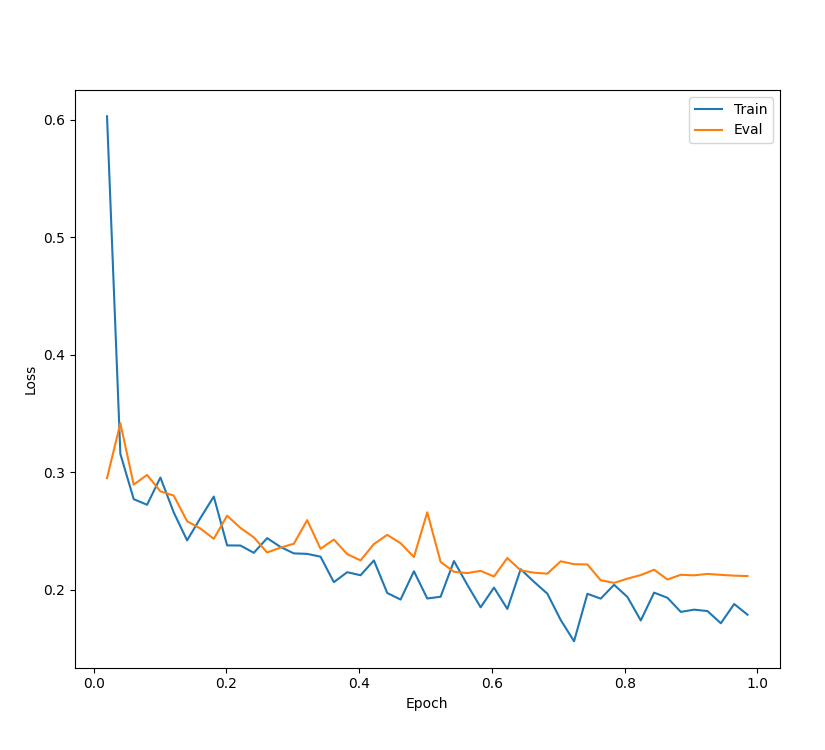
\includegraphics[width=0.95\columnwidth]{loss.png}
\caption{Train and evaluation set loss over 1 epoch.}
\label{fig1}
\end{figure}

\begin{figure}[t]
\centering
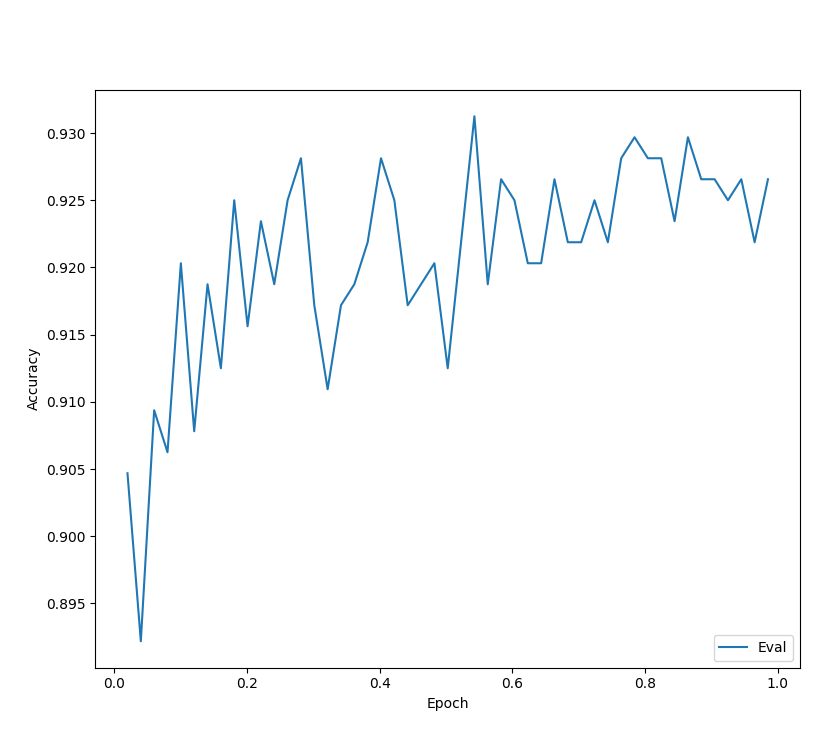
\includegraphics[width=0.95\columnwidth]{accuracy.png}
\caption{Evaluation set accuracy over 1 epoch.}
\label{fig2}
\end{figure}

\bibliography{aaai24}

\end{document}